As can be directly deduced from Table~\ref{tab:gamma}, the smaller values of $\gamma_N$ for a given $\beta$ immediately suggest the higher noise resilience when using floating-point as compared to fixed-point numbers.
\begin{figure}%[h!]
\begin{center} 
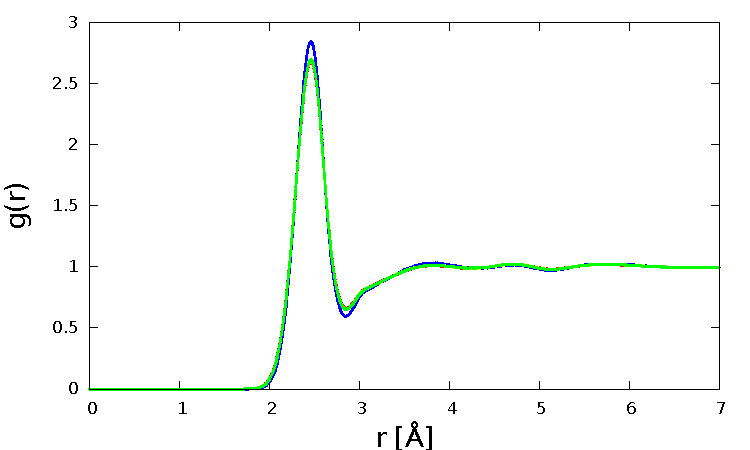
\includegraphics[width=0.475\textwidth]
{figures/fixedpoint.pdf}
\end{center}
\caption{\label{Fig1}
Partial pair correlation function for liquid Si at 3000~K with noisy forces introduced by fixed-point errors of magnitude $10^{-3}$ (green), $10^{-2}$ (yellow) and $10^{-1}$ (blue). For comparison, the results, as obtained by our reference calculations without noise, are shown in red. 
} \end{figure}
In Figs.~\ref{Fig1} and \ref{Fig2}, the Si-Si partial pair-correlation function $g(r)$, as computed using an optimal scheme for orthorombic systems \cite{KAF}, is shown for different values of $\beta$. %In Fig. 1 we show the pair correlation functions g(r) calculated with noisy forces generated from fixed-point errors. In Fig. 2 we show the pair correlation functions g(r) calculated with noisy forces generated with floating-point errors. 
As can be seen, for both fixed-point and floating-point errors, the agreement with our reference calculation is nearly perfect up to the highest noise we have investigated. As already anticipated earlier, the usage of floating-point errors is not only able to tolerate higher noise levels, but is also throughout more accurate. 
\begin{figure}%[h!]
\begin{center}
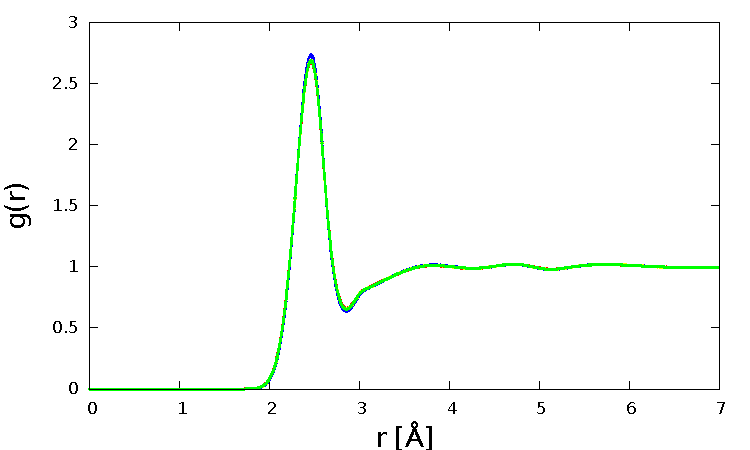
\includegraphics[width=0.475\textwidth]
{figures/floatingpoint.pdf}
\end{center}
\caption{\label{Fig2}
Partial pair correlation function for liquid Si at 3000~K with noisy forces introduced by floating-point errors of magnitude $10^{-2}$ (green), $10^{-1}$ (yellow) and $10^{-0}$ (blue). For comparison, the results, as obtained by our reference calculations without noise, are shown in red. 
} \end{figure}

To verify that the sampling is indeed canonical, in Fig.~\ref{Fig3} the actual kinetic energy distribution as obtained by our simulations using noisy forces and compared to the analytic Maxwell distribution. It is evident that if sampled long enough, not only the mean value, but also the the distribution tails are in excellent agreement with the exact Maxwellian kinetic energy distribution.
\begin{figure}%[h!]
\begin{center} 
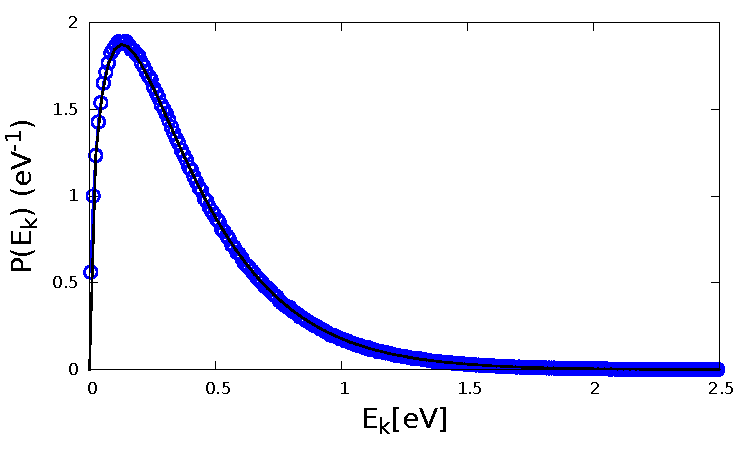
\includegraphics[width=0.475\textwidth]
{figures/maxwelldistribution.pdf}
\end{center}
\caption{\label{Fig3}
Kinetic energy distribution of liquid Si at 3000~K, as obtained by our simulations using noisy forces (blue circles). For comparison the amalytic Maxwell distribution is also shown (red line).
} \end{figure}
To further assess the accuracy of the present method, we expand the autocorrelation of the noisy forces, i.e. 
%\begin{equation}
%\begin{split}
%\left \langle \textbf{F}_{I}^{N}\left ( 0 \right )\textbf{F}_{I}^{N}\left ( t \right )\right \rangle = \linebreak \\ \left \langle \left ( \textbf{F}_{I}\left ( 0 \right ) + \mathbf{\Xi } _{I}^{N}\left(0 \right )\right) \left( \textbf{F}_{I}\left ( t \right )+\mathbf{\Xi } _{I}^{N}\left ( t \right )\right) \right \rangle
%\end{split}
%\end{equation}
\begin{subequations}
\begin{eqnarray}
  && \left \langle \textbf{F}_{I}^{N}\left ( 0 \right )\textbf{F}_{I}^{N}\left ( t \right )\right \rangle \\
  &=& \left \langle \left ( \textbf{F}_{I}\left ( 0 \right ) + \mathbf{\Xi } _{I}^{N} \left(0 \right )\right) \left( \textbf{F}_{I}\left ( t \right )+\mathbf{\Xi } _{I}^{N}\left ( t \right )\right) \right \rangle \\
  &=& \left \langle \textbf{F}_{I}\left ( 0 \right ) \textbf{F}_{I}\left ( t \right )\right \rangle + \left \langle \textbf{F}_{I}\left ( 0 \right ) \mathbf{\Xi } _{I}^{N}\left(t \right )\right \rangle \label{AutoCorr} \\ 
  &+& \left \langle \textbf{F}_{I}\left ( t \right ) \mathbf{\Xi } _{I}^{N}\left(0 \right )\right \rangle + \left \langle \mathbf{\Xi } _{I}^{N}\left(0 \right ) \mathbf{\Xi } _{I}^{N}\left(t \right )\right \rangle.  \nonumber
\end{eqnarray}
\end{subequations}
%\begin{equation}\label{eq:1}
%\begin{split}
%\left \langle \textbf{F}_{I}^{N}\left ( 0 \right )\textbf{F}_{I}^{N}\left ( t \right )\right \rangle = \left \langle \textbf{F}_{I}\left ( 0 \right ) \textbf{F}_{I}\left ( t \right )\right \rangle + \linebreak \\\left \langle \textbf{F}_{I}\left ( 0 \right ) \mathbf{\Xi } _{I}^{N}\left(t \right )\right \rangle +  \left \langle \textbf{F}_{I}\left ( t \right ) \mathbf{\Xi } _{I}^{N}\left(0 \right )\right \rangle + \left \langle \mathbf{\Xi } _{I}^{N}\left(0 \right ) \mathbf{\Xi } _{I}^{N}\left(t \right )\right \rangle
%\end{split}
%\end{equation}
Since the cross correlation terms between the exact force and the additive white noise is vanishing due to Eq.~\ref{CrossCorr}, comparing the autocorrelation of the noisy forces $\langle \textbf{F}_{I}^{N}(0)\textbf{F}_{I}^{N}(t)\rangle$ with the autocorrelation of the exact forces $\langle \textbf{F}_{I}(0) \textbf{F}_{I}(t)\rangle$ permits to assess the localization of the last term of Eq.~\ref{AutoCorr}.
%Since, due to fluctuation-dissipation theorem, the last term of Eq.~\ref{AutoCorr} corresponds to a $\delta$-function, comparing the autocorrelation of the noisy forces $\langle \textbf{F}_{I}^{N}(0)\textbf{F}_{I}^{N}(t)\rangle$ with the autocorrelation of the exact forces $\langle \textbf{F}_{I}(0) \textbf{F}_{I}(t)\rangle$ permits to assess the cross correlation terms between the exact force and the additive white noise. 
The fact that $\langle \textbf{F}_{I}^{N}(0)\textbf{F}_{I}^{N}(t)\rangle$ is essentially identical to $\langle \textbf{F}_{I}(0) \textbf{F}_{I}(t)\rangle$, as can be seen in Fig.~\ref{Fig4}, implies that $\langle \mathbf{\Xi } _{I}^{N}(0) \mathbf{\Xi } _{I}^{N}(t)\rangle$ is very close to a $\delta$-function as required by the fluctuation-dissipation theorem in order to ensure an accurate canonical sampling of the Boltzmann distribution. 
\begin{figure}%[h!]
\begin{center}
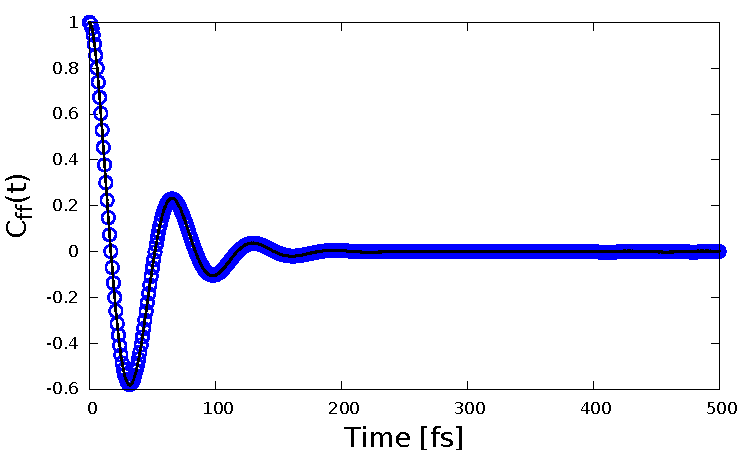
\includegraphics[width=0.475\textwidth]
{figures/force_autocorrelation.pdf}
\end{center}
\caption{\label{Fig4}
The Autocorrelation of the noisy forces \(
\left \langle \textbf{F}_{I}^{N}\left ( 0 \right ) \textbf{F}_{I}^{N}\left ( t \right )\right \rangle \)(line), which are compared to the autocorrelation of the exact forces \( \left \langle \textbf{F}_{I}\left ( 0 \right ) \textbf{F}_{I}\left ( t \right )\right \rangle \)(circles). 
} \end{figure}

%If the random value that was used to generate the computational error is chosen in the range [0,1] instead of [-0.5,0.5], we encounter a phenomenon called "Flying Ice Cube" \cite{flyingIceCube} during our MD simulations.  
